The Blender software (www.Blender.org) was chosen as the simulation environment for our project. Blender is a free, open source program designed for 3D modeling, physics simulation, and game design. Blender provides a means of easily creating 3D objects, attaching properties and constraints to those objects, and developing scripts that interact with the software.

Object models in Blender are stored as “objects” with associated “meshes.” A mesh is a data structure with a series of faces, edges, and vertex locations in space for the object. Blender also contains methods for adding custom properties to objects, which serves to make the system quite extensible. Native support for 3D modeling and operations was highly desirable as well, as 2D approaches considered possessed limited support for modeling and manipulating three-dimensional environments. With Blender’s existing 3D support and extensive library utilities for 3D object management, the task of developing a simulation environment was eased considerably.

Blender contains a very accessible Python API. This allows python scripts to access methods in Blender, and can allow the system to create and change objects, measure properties of the above objects, and even instantiate physical laws (such as gravity) in the scene. The direct purpose of this system is to perform the following function: EPILOG will communicate with a built in series of Python scripts, which then, in turn, will utilize Blender to construct a 3D environment, which can then be examined to derive information about the scene to be fed back as input into EPILOG. These functions are to be performed incrementally, i.e., in support of a sentence-by-sentence story understanding process. 

The Mental Imagistic Reasoning System, “MIRS” exists as a series of python files and a database of objects which interface with Blender. The source folder contains three python files: Classes.py, predMethods.py, and obutils.py, and a single directory: ObjectData.

Classes.py file is the highest level python file, and serves as the top level of the system’s organization and control. Classes.py contains three classes: Scene, Entity, and Predication. 
	
The Scene class serves to hold the information currently being modeled in the blender scene, and to provide methods for adding entities and predications to the scene, and for querying the scene for how well a given predication is satisfied. Although object placement in the system is meant to ensure that all the predications in a given scene are satisfied, this is not necessarily the case.
	
Each instantiation of the Entity class stands for an entity in the domain of the scene being modeled. The Entity class contains attributes for storing information about the given entity - including a pointer to the object being modeled in the Blender scene - and methods for interacting with the object in the blender scene.
	
Each instantiation of the Predication class stands for a predication active in the current scene. A Predication instance contains references to the blender [parent] objects bound by the given predication, and a method for returning placement constraints for either of the objects relative to the other, and one for querying how well the predication is satisfied given the current locations/orientations of the Predication’s objects in the Blender scene. The Predication class is generic, and imports placement and querying methods specific to a given Predication (e.g. “near”, “above”) from the predMethods.py file. Note that the actual functions for the predication are stored as variables in each class instantiation. Once the methods are copied from predMethods.py, predMethods.py is no longer called directly by the predication.

predMethods.py contains placement and query methods for each predicate, for example (respectively) nearP and nearQ for the “near” predicate. Many of these predicates involve complex functions in Blender’s three-dimensional space, which are stored in obutils.py.

obutils.py consists of various methods for operating on Blender objects, and is used by both predMethods.py and Classes.py.

The ObjectDatabase directory contains two sub-directories: OBJ and XML. These correspond, respectively, to the two types of information being stored for each object: the three-dimensional model of the object as used by Blender, and other information about the object that is not directly used by Blender. 

In the SRS, entities are modeled in Blender not with a single mesh, but with separate meshes corresponding to each of the entity’s parts. When an entity’s meshes are imported to the scene, the Entity class imports entity ‘.obj’-format object files from the ‘item name’ subdirectory in the OBJ directory, where ‘item name’ stands for the entity’s key (e.g. “person” or “house”). In the Blender scene, these part meshes are bound as children under an empty-point Blender object that is the parent. In the Entity class, the pointer to the Blender object is a pointer to this empty parent object (from which children/parts are easily accessed).

\begin{wrapfigure}{r}{0.5\textwidth}
	\begin{center}
		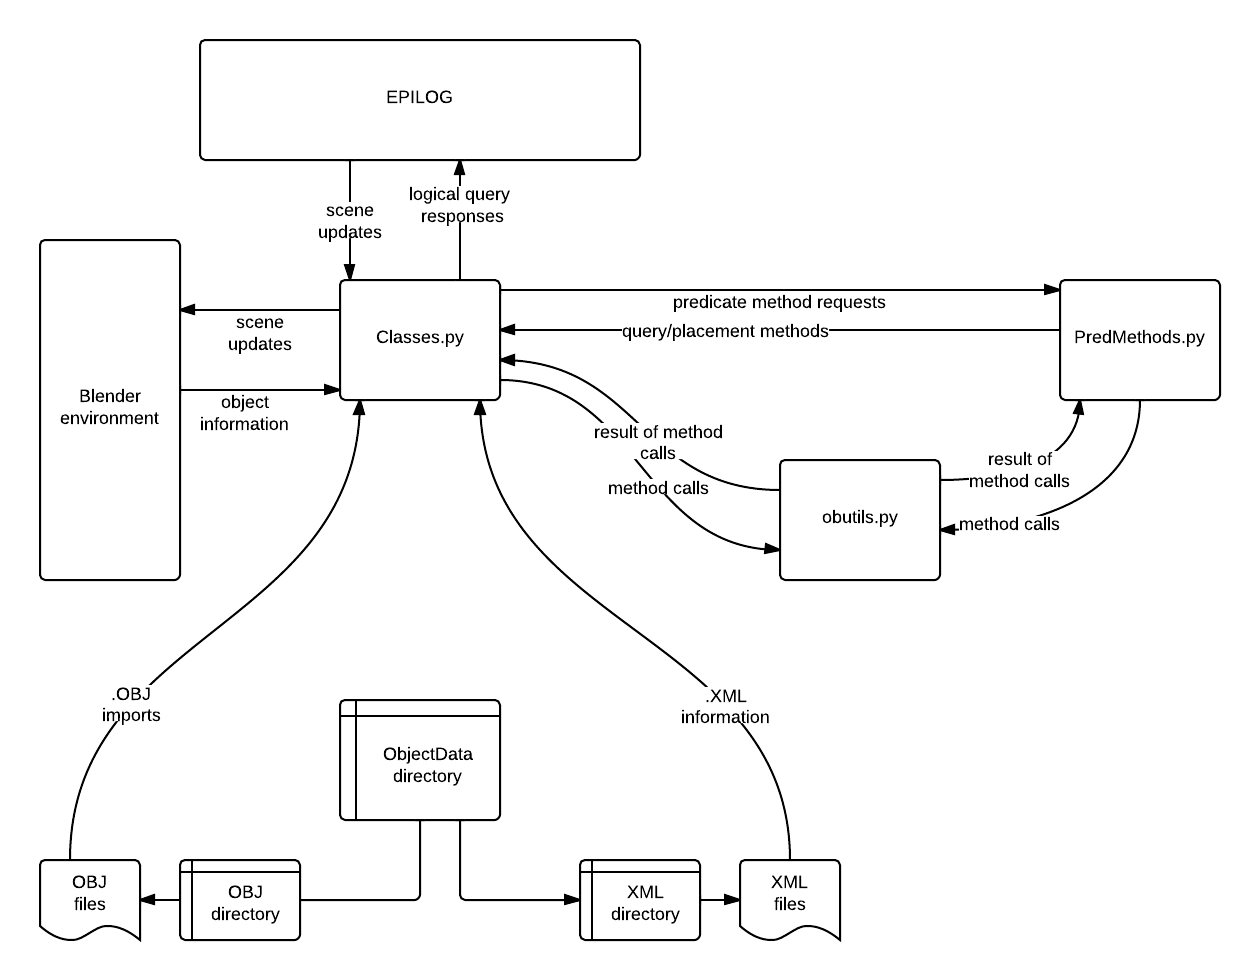
\includegraphics[width=0.48\textwidth]{figures/mirs_flow.png}
	\end{center}
	\caption{Human and AI agents have similar move optimality across all tests.}
\end{wrapfigure}

The XML directory contains ‘item name’.xml files for each entity for which there exist Blender models, where ‘item name’ stands for the entity's key. Each XML file contains the following information: a meronomy graph for the entity, a list of the parts with meshes (for example, a person’s “arm” may not have a corresponding mesh, while their “forearm” and “upper arm” do), and finally bounding box coordinates for the object. 

Periodic updates, predominantly introduction so new objects and predications, as well as changes to existing objects and predications, are sent to the specialist by EPILOG.

My particular work for both this independent study and the project as a whole focused on the construction of the predicate class, as well as the helper methods in obutils.py, and management and organization of the program files. As such, these elements (rather than the entire project) are listed below.

\begin{longtabu}{| p{5cm} | p{10cm} |}
	\cline{0-0}
	obutils.py  \\\hline
	Methods & Descriptions \\\hline
	
	cast\_thru(Object start\_obj,Vector endpt, Object end\_obj) & Casts repeated rays from start\_obj to endpt, noting the degradation due to occlusion that occurs along the way stopping when end\_obj is hit. Returns a value 0-1 indicating the occlusion encountered on the way \\\hline
	
	nudge(Object a, Vector pt) & Returns a points several thousandths closer to object A from pt, used in repeated ray casting experiments \\\hline
	
	rayCast(Object a,Vector b) & Shoots a ray from the center of object a to b, returns the same as Scene.ray\_cast(start,end) \\\hline
	
	alignMeasure(a,b,top=float(inf), right=float(inf),
	bottom=float(-inf), left=float(-inf)) & Creates a rectangular prism mesh on top of b that can be used for intersection testing. If no maximum top/bottom/etc... points are specified it will use the most outward points on b's bounding box \\\hline	
	
	highest(Object obj,char dim) & Returns the highest vertex in the object (in the dimension (x,y,z) specified) \\\hline
	
	lowestPt(Object obj,char dim) & Returns the highest vertex in the object (in the dimension (x,y,z) specified) \\\hline
	
	Returns the highest vertex in the object (in the dimension (x,y,z) specified) & Returns the part of m's mesh that is intersecting with a \\\hline
	
	getDiff(Object m, Object a) & Returns the part of m's mesh that is not intersecting with a \\\hline
	
	closest\_points(Scene scene,Object a,Object b) & Returns a tuple containing the closest point on the mesh of a to b, and the closest point to a on b's mesh, in that order \\\hline
	
	maxDim(Object [] ary) & Returns the largest dimension (x,y,z) among all objects in ary \\\hline
	
	distance(Vector a, Vector b) & Returns the distance between a and b (will not work if an object is in the way). Measured without pathfinding. \\\hline
	
	def glob2Loc(Vector pt,object obj) & Returns point pt in object obj's local space \\\hline
	
	vertsGlob(Object obj) & Returns an array of obj's vertices in global coordinates \\\hline
	
	locs2Glob(Vector[] pts, Object obj) & Returns the location of the coordinates in pts in global coordinates (assuming pts are originally in obj's local space) \\\hline
	
	loc2Glob(Vecotr pts, Object obj) & Same as locs2Glob, but for only one point \\\hline
	
	aInBSpace(Vector pt, Object a, Object b) & Returns pt (which is in a's local space at the start) in b's local space; works through matrix multiplication \\\hline
	
	getVolume(Object obj) & Returns the volume in $BV^3$ of the object; underneath this wrapper method are numerous helper methods \\\hline
\end{longtabu}

Each Predication instance contains two methods: Place() and Query(). These predicates are stored as <predicate name>P and <predicate name>Q. As shown above, the placement function of the near predication is nearP and the query function is nearQ. Query methods evaluate the scene and return a value for how well the given predicate is satisfied in the current scene. This can be done continuously as a value between 0.0 and 1.0, or as a boolean. For a boolean value, the continuous answer is still evaluated: 1.0 is returned if the answer is above 0.5, and 0.0 if below. The purpose of the BinaryFlag attribute in the Predication class is to determine whether the predicate is evaluated as a boolean value or not.

Place() should return the areas in the Blender scene where the predicate holds true for one entity relative to the other. This makes the assumption that the second object has already been placed; for example in the predication ‘near(A,B)’, if Place(A) was called, it would return an acceptance area of ‘nearness’ for A, such that the predication is satisfied. At present, our placement locations are returned as a tuple of pairs, with each pair containing the minimum and maximum values for the x, y, and z dimensions. This format of object placement has fundamental issues and should be replaced with a different format. Because of this limitation, very few predicates currently have functioningl Place() methods, and so the table below only lists Query() methods.

\begin{longtabu}{| p{2.5cm} | p{2.5cm} | p{7cm} | p{4cm} |}
	\cline{0-0}
	predMethods.py  \\\hline
	Predicate & Description & Query & Place) \\\hline
	
	near(A,B) & determines whether A is close to B & iterates through the children of a and b and selects the two with the shortest distance between the two meshes. the value returned is the distance relativized to the sizes of the two entities. The result is not proportional to distance, and returns true up to a certain distance and then a result from a steeply graded exponential function thereafter. & obutils.maxDim()
	obutils.closestPoints()
	obutils.isArbitrarilyLarge()
	\\\hline
	
	under(A,B) & determines to what extent A is underneath B & draws a temporary object directly under B; the percent volume of A that intersects with this is the return value & obutils.alignMeasure()
	obutils.getIntersection()
	obutils.getVolume()
	obutils.deleteObject()
	\\\hline
	
	in(A,B) & determines whether A is inside B’s bounding box & draws a temporary object around B’s bounding box and returns the percent volume of A, or true if more than half of A’s volume is in B. & obutils.getVolume()
	obutils.deleteObject() \\\hline
	
	inside(A,B) & determines the extent to which A is inside B & same as in(A,B), but the temporary object is drawn around B’s mesh rather than bounding box & obutils.getIntersection()
	obutils.getVolume()
	obutils.deleteObject() \\\hline
	
	above(A,B) & determines the extent to which A is above B & Draws a temporary object in the space above B and returns the percent of A’s volume that intersects. & obutils.alignMeasure()
	obutils.getIntersection()
	obutils.getVolume()
	obutils.deleteObject() \\\hline
	
	isTouching(A,B) & determines the extent to which A is touching B & This function works the same as near(A,B), but does not adjust with relative object size and requires objects to be much closer. & obutils.distance() \\\hline
	
	canSee(A,B) & determines whether A can “see” B & (this assumes an “eye” object on A). Ray casting is done from A’s eye to points on the meshes of B’s children. The percent of successful casts (that reach B) is the value returned. If the cast hits a translucent object, it will continue but will return a reduced value
	 & obutils.cast\_thru() \\\hline 
\end{longtabu}